\subsubsection{4-Line Vertices}
\begin{itemize}
    \item There is no complete list of all possible 4-line vertices. 
    \item As seen in \cref{fig: feynman_diagram_vertices}, we know that both gluons, Higgs bosons and $W / Z / γ$  bosons can have 4-line vertices. This means two particles can scatter, creating two new particles, without an intermediate particle.
    \item This is caused by particles being able to interact with themselves. 
    \item These are rarely used
\end{itemize}

\subsection{Creating Feynman Diagrams}
Often there are multiple ways to describe the same process. There can be multiple different time orders. Example can be seen in \cref{eq: moeller_scattering}, visualized in two different ways in \cref{fig: moeller_scattering}. This is not always done as it is implied that both are possible, and you need to calculate both. A time independent version can be seen in \cref{fig: moeller_scattering_time_independat}.

\begin{equation}\label{eq: moeller_scattering}
    e^{-} e^{-} → e^{-} e^{-}
\end{equation}

\begin{figure}[ht!]
\centering
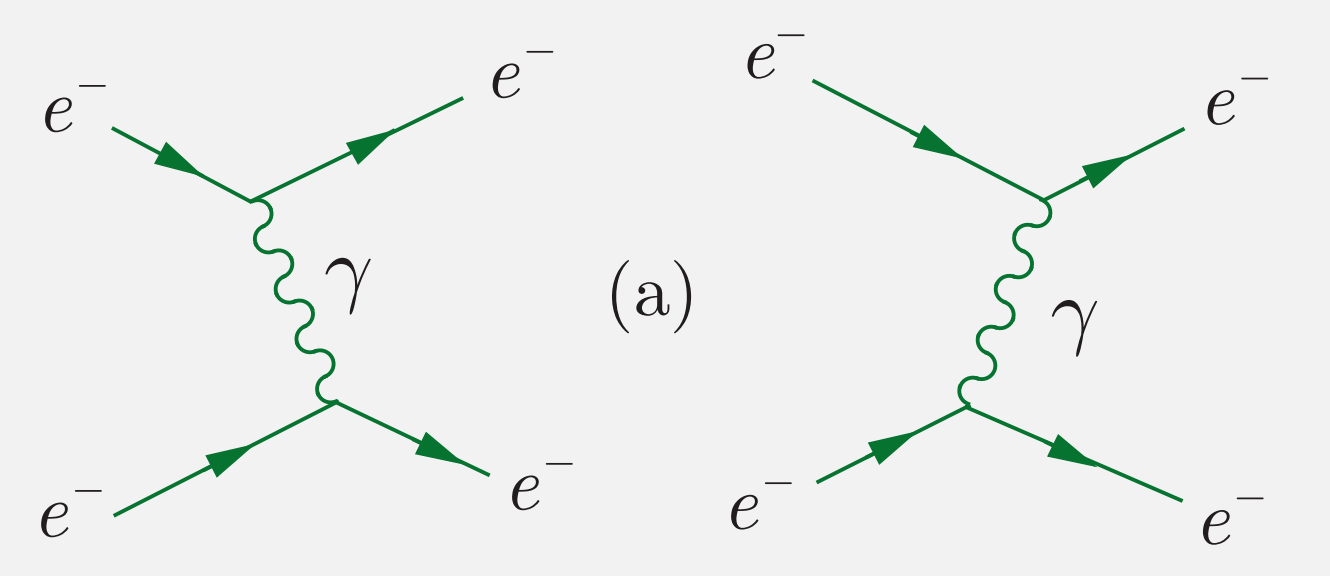
\includegraphics[width = .75\textwidth]{moeller_scattering.png}
\caption{Two different ways to visualize Møller scattering as seen in \cref{eq: moeller_scattering}.}
\label{fig: moeller_scattering}
\end{figure}

\begin{figure}[h!]
\centering
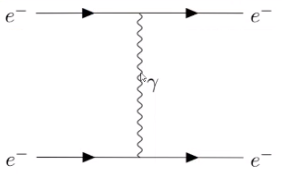
\includegraphics[width = .6\textwidth]{moeller_scattering_time_independat.png}
\caption{A time independent version of Møller scattering as seen in \cref{eq: moeller_scattering}.}
\label{fig: moeller_scattering_time_independat}
\end{figure}


\subsubsection{Tip for Choosing Time-Ordering}
Just pick one and see if the charge and all other properties are conserved. As seen in \cref{fig: time_ordering_example}, we can choose the time ordering based on the charge conservation. Only the electron can emit the negatively charged $W^{-}$-boson. Therefore, the emission on the bottom happens before absorption on the top. The unambiguous time ordering can be seen in \cref{fig: time_ordering_example_solved}. We could of course have flipped the figure horizontally. 

\begin{figure}[h!]
\centering
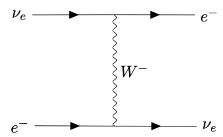
\includegraphics[width = .6\textwidth]{time_ordering_example.png}
\caption{Example showing a case were logic is used to choose the time ordering.}
\label{fig: time_ordering_example}
\end{figure}

\begin{figure}[h!]
\centering
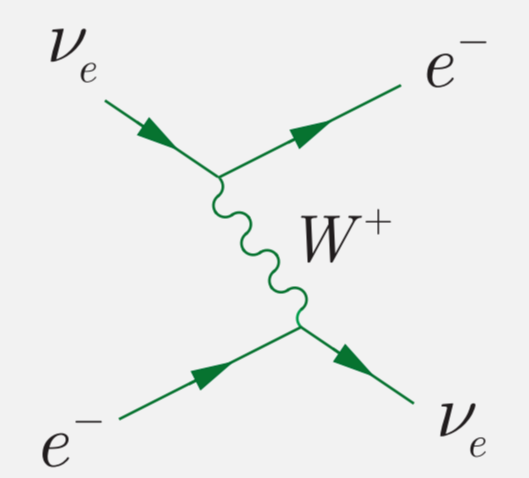
\includegraphics[width = .6\textwidth]{time_ordering_example_solved.png}
\caption{Solved case of ambiguity in time ordering from \cref{fig: time_ordering_example}.}
\label{fig: time_ordering_example_solved}
\end{figure}

\subsubsection{Current interactions}
\begin{itemize}
    \item Fermion lines must be continuous. 
    \item Anti-fermion lines must be continuous.
\end{itemize}

\section{Relativity and Anti-Particles}
\subsection{Dirac Equation}
\begin{itemize}
    \item A relativistic equation for the electron.
    \item Makes a prediction of the positron (anti-electron). 
    \item All charged particles have an anti-particle $(p, \bar{p})$, $(μ^{-}, μ^{+})$
    \item For neutral particles, their respective anti-particles have the same charge, but their quarks are opposites (neutrons), or they are their own anti-particle (photons).
    \item Predicts a relation between spin $\vec{S}$ and magnet moment $\vec{μ} = \vec{qS} / m$. This has been confirmed for the electron and muon, but not for protons and neutrons. This hints at the existence of substructure in protons and neutrons.
\end{itemize}

\subsection{Symmetries and Conservation Laws}
\subsubsection{Symmetries and Conserved Quantities}
Noethers theorem states that for every continuous symmetry, there is a conserved quantity. A list of symmetries and their conserved quantities can be seen in \cref{tab: symmetries_table}. They all have their quantum operators. If the physics remains unchanged under a transformation, the system is said to be symmetric under that transformation.

\begin{table}[h!]
\centering
\begin{tabular}{ |c|c|c| }
    \hline
    \textbf{Symmetry} &\textbf{Conserved Quantity} &\textbf{Interactions} \\ 
    \hline
    Space translation &Linear momentum &All \\ 
    Space rotation &Angular momentum &All \\ 
    Time displacement &Energy &all \\ 
    Space inversion &Parity &Not weak \\ 
    Charge inversion &C-parity &Not weak \\ 
    u <-> d &Isospin &String \\ 
    \hline
    \end{tabular}\label{tab: symmetries_table}
\end{table}

\subsubsection{Intrinsic Parity}
\begin{itemize}
    \item All particles at rest have intrinsic parity. This comes from a the only eigenvalue of the parity operator $\hat{P}$ acting on a plane wave function $Ψ(\vec{r},t) = \exp \left(i(\vec{r} ⋅ \vec{p} - Et) / h\right)$, can only return the same wavefunction if $\vec{p} = 0$. 
    \item By convention, we say fundamental fermions have $P = +1$, and their antiparticles have $P = -1$. This is arbitrary. 
\end{itemize}

\subsubsection{Parity of Bound States}
In quantum mechanics we can split the spatial part of the wave function into a radial part $R(r)$ and a spherical harmonic $Y_{l}^{m}(\theta, \phi)$. 
\begin{equation}
Ψ = R_{nl}(r) Y_{l}^{m}(\theta, \phi)
\end{equation}
\begin{equation}
\vec{r} → - \vec{r} \quad ⇒ \quad  r → r, θ → π - θ, ϕ → ϕ + π
\end{equation}
The parity of the spherical harmonic is $(-1)^{l}$. 

\subsubsection{Charge Conjugation}
\begin{itemize}
    \item The charge conjugation operator $\hat{C}$ changes all particles to their antiparticles.
    \item Eigenstates of $\hat{C}$ are particles that are their own antiparticles, like photons. 
    \item Eigenvalues are $\pm 1$. 
\end{itemize}

\subsubsection{Natural Units}
\begin{itemize}
    \item To make life simple we let $ℏ = c = 1$, and only add them back at the end when knowing the units. 
    \item All quantities are measured in energy $\left(eV\right)^{n}$. 
    \item Energy: $eV$
    \item Momentum: $eV / c$
    \item Mass: $eV / c^2$
    \item Time and length: $1 / eV$
    \item It is useful to memorize $ℏc ≈ 197 MeVF$
\end{itemize}

\subsection{Scattering}
\begin{itemize}
    \item Scattering experiments is the core of nuclear and particle physics. 
    \item Elastic Scattering: Same particles in the initial and final state. An example can be seen in \cref{eq: elastic_scattering_example}, where a proton and electron collide. The electron might lose some energy in the form of momentum to the proton, but the particles are the same and their center of mass is unchanged. 
    \begin{equation}\label{eq: elastic_scattering_example}
        e^{-} p → e^{-} p
    \end{equation}
    \item Inelastic Scattering: Different particles in the initial and final state. An example can be seen in \cref{eq: inelastic_scattering_example}, where a particle can collide with an atom and excite it to a higher energy state.
    \begin{equation}\label{eq: inelastic_scattering_example}
        a A → a + A^{*}
    \end{equation}
\end{itemize}

\subsubsection{Decay}
\begin{itemize}
    \item Unstable parent particles decay into stable and lighter daughter particles. 
    \item Atom decay: $A^{*} → A + γ$
    \item Neutron decay: $n → p + e^{-} + \bar{ν}_{e}$
    \item $Z^{0}$ boson decay: $Z^{0} → e^{+} + e^{-}$. 
    \item For free particles, we must have a positive Q-value defined in \cref{eq: Q_value}.
    \begin{equation}\label{eq: Q_value}
        Q = \left(M_{\text{P}} - ∑_{i}^{} M_{\text{D}_i}\right)c^2
    \end{equation} 
    \item For unstable nuclei and particles we have a decay rate as seen in \cref{eq: decay_rate}.
    \begin{equation}\label{eq: decay_rate}
        \frac{dN(t)}{dt} = -λN(t)
    \end{equation}
    The decay constant $λ$ is related to the half-life $T_{1/2}$ by $λ = \ln(2) / T_{1/2}$, with units of $s^{-1}$. 
    \item The mean lifetime is given by $τ = 1 / λ$. This represent the average time a particle will live before decaying. The mean lifetime refer to the rest frame of the particle. 
    \item Decay Width $Γ$: The decay rate in natural units. It is related to the decay constant by $Γ = ℏλ$.
    \item Decay Channels: The different particles a particle can decay into. Each has its own decay width, where the total decay width is the sum of all the decay widths $Γ = ∑_{i}^{} Γ_i$. Each channel has the same mean lifetime. They live for the same amount of time, but the probability of decaying into a specific channel is different. 
    \item Branching Fraction: The probability of a particle decaying into a specific channel, given by $B = Γ_{i} / Γ_{\text{tot}}$.
\end{itemize}

\paragraph{Tau Particle}
\begin{itemize}
    \item A heavy particle which always decays ($B = 100 \%$).
    \item A list of some decay channels, responsible for approximately $60 \%$ of all decays:
    \begin{itemize}
        \item $B(τ^{-} → e^{-} \bar{ν}_{e} ν_{τ}) = 17.8 \%$
        \item $B(τ^{-} → μ^{-}\bar{ν}_{μ} ν_{τ}) = 17.4 \%$
        \item $B(τ^{-} → π^{-} π^{0} ν^{τ}) ? 25.5 \%$
    \end{itemize}
\end{itemize}

